\documentclass[a4paper,12pt]{article}
\usepackage[compact]{titlesec}
% `fontset=none` means forbidden default the font setting
\usepackage[UTF8, fontset=none]{ctex} % cjk
\usepackage[margin=0.79in]{geometry} % layout
\usepackage{amsmath, amssymb} % math
\usepackage{fancyhdr} % head and footer
\usepackage{lastpage} % get total page number
\usepackage{xifthen} % enhanced if-else condition
\usepackage{multirow} % merge table item
\usepackage{tabularx} % enhanced table
\usepackage{afterpage} % add table at the second page
\usepackage{tabularray} % enhanced table 2
\usepackage{titlesec} % custom title format
\usepackage{indentfirst} % custom section ident
\usepackage{enumitem} % custom item
\usepackage{listings} % source code
\usepackage{graphicx} % figure
% \usepackage{pgffor} % for-loop
% \usepackage{totcount} % counter

% % register counter
% \regtotcounter{section}
% \newcounter{sectioncount}

% font setting
\setmainfont{Times New Roman}
\setmonofont{Consolas}
\setCJKmainfont{SimSun}[AutoFakeBold]
\setCJKsansfont{SimHei}[AutoFakeBold]
\setCJKmonofont{FangSong}[AutoFakeBold]
\setCJKfamilyfont {zhkai} {KaiTi}
\NewDocumentCommand \kaishu{}{\CJKfamily{zhkai}}
% get current semester
\newcommand{\currentsemester}{
  \ifnum\month<10
    1
  \else
    2
  \fi
}

\newcommand{\school}{上海交通大学}
\newcommand{\papertype}{A}
\newcommand{\startyear}{\the\year}
\newcommand{\nextyear}{\the\numexpr\startyear+1\relax}
\newcommand{\semester}{\currentsemester}
\newcommand{\coursename}{操作系统}

% header and footer
\pagestyle{fancy}
\fancyhf{} % clear the default config
% header
\renewcommand{\headrulewidth}{0.4pt}
\renewcommand{\headrule}{\hrule width\textwidth height\headrulewidth}
% footer
\fancyfoot[C]{
  \footnotesize
  \underline{\ \papertype\ } 卷 \space
  第 \underline{\ \thepage\ } 页 \space
  共 \underline{\ \pageref{LastPage}\ } 页
}

% custom section format
\renewcommand{\thesection}{\chinese{section}}
\titleformat{\section}
  {\normalfont\Large\bfseries}
  {\thesection、}
  {0pt}
  {}

% custom subsection format
\renewcommand{\thesubsection}{\arabic{subsection}}
\titleformat{\subsection}[runin]
  {\normalfont\large\bfseries}
  {\thesubsection.\ }
  {0pt}
  {}

% custom subsubsection format
% \setcounter{sectioncount}{\number\totvalue{section}}
\renewcommand{\thesubsubsection}{\arabic{subsubsection}}
\titleformat{\subsubsection}[runin]
  {\normalfont\bfseries}
  {\thesubsubsection)\ }
  {0pt}
  {}

% subsubsection indent
\titlespacing{\section}{0em}{1em}{0pt}
\titlespacing{\subsection}{0pt}{0.25em}{0.5em}
\titlespacing{\subsubsection}{1em}{0.25em}{0.5em}

% paragraph space
\setlength{\parskip}{0.5em}

% custom list
\setlist[itemize]{
    itemsep=0.20em,
    parsep=0em,
    topsep=0.20em,
    partopsep=0.20em
}

\setlist[enumerate]{
    itemsep=0.20em,
    parsep=0em,
    topsep=0.20em,
    partopsep=0.20em
}

% source code
\lstset{
	basicstyle=\small\ttfamily,,
  numbers=left,
  breaklines=true,
  extendedchars=true,
  frame=single,
  framesep=1pt,
  float,
  linewidth=0.8\linewidth,
  framexleftmargin=0.5em,
  framexrightmargin=0.5em,
  lineskip=0.1em
}

% score command
\newcommand{\score}[1]{(#1')}

\begin{document}

% title
\begin{center}
  \zihao{4} \school 试卷(\underline{\papertype} 卷)\\
  \zihao{5} (\underline{\ \startyear\ } 至 \underline{\ \nextyear\ } 学年 第 \underline{\ \semester\ } 学期) \\
  \vspace{0.5cm}
  \zihao{5}
  \begin{tabularx}{0.9 \textwidth}{XXX}
    班级号:\underline{\hspace{0.15 \textwidth}} & 学号:\underline{\hspace{0.2 \textwidth}} & 姓名:\underline{\hspace{0.2 \textwidth}} \\
    \multicolumn{2}{l}{课程名称:\underline{\makebox[0.43 \textwidth][l]{\hfill \coursename \hfill}}} & 成绩:\underline{\hspace{0.2 \textwidth}} \\
  \end{tabularx}
\end{center}


% commitment
\afterpage{
  \noindent
  \begin{minipage}{0.22 \textwidth}
    \zihao{5}
    \kaishu \hspace{2em} \textbf{我承诺,我将严格遵守考试纪律。}
    \vspace{2.5em}

    承诺人:\underline{\hspace{0.5 \textwidth}} \\
    \vspace{1em}
  \end{minipage}
  \hfill
  \begin{minipage}{0.73\textwidth}
    \begin{tblr}{
      colspec = {|X[3,l]|X[c]|X[c]|X[c]|X[c]|X[c]|X[c]|X[c]|X[c]|X[c]|},
      rows = {ht=10mm},
      hlines,
      vlines,
      }
      \textbf{题号} & & & & & & & & & \\
      \textbf{得分} & & & & & & & & & \\
      \textbf{批阅人} & & & & & & & & & \\
    \end{tblr}
  \end{minipage}
  \vspace{2em}
}


% \foreach \i in {1,2,3,4,5,6,7,8,9} {
% \&
% \ifnum\i>\value{sectioncount} % 比较数值而非计数器
%   0
% \else
%   \i
% \fi
% }
% TODO: 分数计算
% TODO: 代码块和图片样式
% TODO: 答案编辑

\section{内存抽象 \score{36}}

\subsection{}

虚拟内存技术的出现改变了程序员编写应用程序时的基本假设,为用户态程序提供了大量独占连续内存的假象,极大地方便了开发。

\subsubsection{}

TLB 的作用是什么?如果使用单级页表还需要 TLB 吗?\score{4}

\subsubsection{}

当操作系统选择 4KB 作为最小页大小时, L2 页表项和 L1 页表项对应大页的页面大小分别为 2MB 和 1GB。
那么当操作系统选择 16KB 或 64KB 作为最小页大小时,对应大页(只考虑 L2 页表项)的页面大小是多少?请写出计算过程。\score{4}


\subsection{}

伙伴系统( buddy system )是一种高效的内存分配器算法,其本质是一种可以快速分裂和合并空闲块的分离空闲链表。(“空闲链表 x ” 表示每一块有 $2^{x}$ 个页)

\subsubsection{}

假设伙伴系统初始只有一块 64KB 大小的内存块,保存在空闲链表 4 当中。依次分配 30KB、9KB、4KB 三次内存后,请问空闲链表 0~3 各剩几个空闲块?\score{4}

\subsubsection{}

伙伴系统会存在内部碎片的问题,请说明内部碎片是什么,并计算第一问中存在多大的内部碎片。\score{4}


\subsection{}

某厂商为用户提供云服务,在单一服务器上运行了大量虚拟机同时服务不同用户,这些虚拟机中有很大一部分运行着相同的操作系统和相同的应用程序。
为了提升服务器的资源利用率和整体性能,该厂商计划通过内存去重技术来减少内存的占用。

\subsubsection{}

请根据你所学的虚拟内存管理的知识,简要说明内存去重的基本原理。\score{4}

\subsubsection{}

在该厂商使用了内存去重技术后,部分用户反馈云服务的质量下降,请求的平均延迟增加,请推测可能的原因是什么?\score{4}

\subsubsection{}

部分用户认为内存去重技术可能危害自己的数据安全,请推测原因。\score{4}

\subsection{}

小明开发了一款单线程的服务器应用,希望提升应用处理请求的性能,于是在原有基础上将应用修改为四线程运行,结果并没有得到四倍的性能提升。
经过详细的性能分析和监控,他发现以下现象: CPU 利用率低、CPU 缓存命中率低、锁争用少。进一步分析发现,单线程版本应用定义了一个频繁访问和修改的全局数组,改为四线程将数组规模扩大为四倍,每个线程访问其中的一部分。

\subsubsection{}

请解释为什么在这种情况下会出现CPU利用率低和缓存命中率低的现象。\score{3}

\subsubsection{}

请提出至少两种解决方案解决该问题。\score{3}


\section{系统安全 \score{16}}

\subsection{}

如果允许且只允许你修改一台正在运行中的计算机内存中的任意一个 bit ,你该如何获取到最高权限?简述不少于 2 种方案。\score{4}

\subsection{}

从安全的角度分析,为什么对文件操作不使用 inode 号作为参数而要用 fd 作为参数?不少于 2 种原因。\score{4}

\subsection{}

现在当拥有一台 Copilot+ 电脑,用户可以在电脑上开启微软最新推出的 Recall 功能。
Recall 是结合了 Copilot 学习、理解、推理能力应运而生的「回溯」技术,即利用大模型不断追踪用户在 Windows 上的操作,每隔几秒就会给用户的屏幕拍摄一张快照,
在用户需要时,输入一段文字,它将利用过去的任何线索进行搜索,以时间线的形式回放操作,允许用户浏览过去的活动,包括应用、文档和网站。

\subsubsection{}

过去潜在的黑客大费周章却只能针对单一应用攻击,但现在他们或许有机会一次性从你的电脑中获得最近一小时甚至一个月的操作记录,如何避免这样的事情发生?
不少于 3 点(可从系统安全保护层次、文件安全性隔离性保护、应用隔离等方面回答)。\score{4}

\subsubsection{}

Recall 在拍摄快照时,并不会隐藏密码或重要帐号等信息,它甚至已经记录下你的所有隐私操作。
请你选择课程中介绍的访问控制策略,设计一个允许用户控制的 Recall 启用方案,允许用户决定操作是否允许被 Recall 记录,并确保记录下的数据被安全使用。\score{4}

\section{系统虚拟化 \score{28}}

\subsection{}

DMA 允许外设直接访问内存,无需通过 CPU 进行数据传输,提高吞吐的同时减少 CPU 负载。这也给恶意外设提供了可乘之机,恶意外设可以通过 DMA 读写不被允许访问的内存。

\subsubsection{}

请简述 IOMMU 是如何解决这个问题的。\score{4}

\subsubsection{}

在生产实践中, IOMMU 往往会配置 2MB 或更大的页,请问有什么好处?\score{4}

\subsection{}

持续运行的 fork bomb 会最终消耗掉 OS 所有计算资源,内存资源和 PID 资源。

\subsubsection{}

PID namespace 是否能抵御 fork bomb 对容器的攻击,为什么?\score{4}

\subsubsection{}

在虚拟机中运行的 fork bomb 会对宿主机造成什么样的影响,为什么?\score{4}

\subsection{}

写时复制( Copy on Write, CoW )技术通过延迟复制优化性能,一般通过将 page table entry (PTE)的 read only bit 设置为 1 实现。

\subsubsection{}

如果 hypervisor 想让多个虚拟机以 CoW 的形式共享同一块物理内存,应该将哪一阶段页表对应的 PTE 的 read only bit 设置为 1 ? \score{3}


\subsubsection{}

当虚拟机的某个进程试图写入被 hypervisor 映射为 CoW 的内存时,请描述从尝试写入到完成写入的过程。\score{3}

\subsection{}

ChCore Lab 使用 \verb|qemu-system-aarch64| 在助教提供的 x86-64 的 Linux 虚拟机上模拟树莓派 3 的执行环境。请问这里的 \verb|qemu-system-aarch64| 更可能使用二进制翻译,半虚拟化和硬件虚拟化的哪一种方法进行计算虚拟化?说明判断理由。\score{3}

\subsection{}

在二阶段页表翻译过程中,如果第一阶段用 4KB 页表( 4 级),第二阶段用 2MB 页表( 3 级),在 TLB miss 的情况下,将 \verb|GVA| 翻译为 \verb|HPA| 最多需要几次访存?说明计算过程。\score{3}


\section{同步原语 \score{20}}

\subsection{}

Barrier 用于协调多个线程,使它们在执行到某个特定点时等待,直到恰好 K 个线程都到达该点后再继续执行,其中 K 是 barrier 初始化时设定的值。
下面展示了一个 barrier 的实现:

\begin{figure}[!htb]
  \centering
  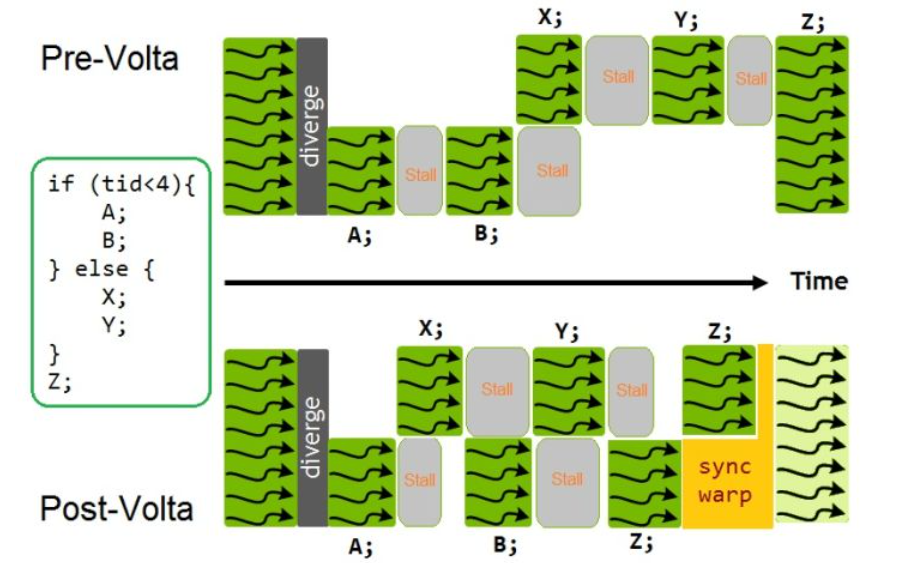
\includegraphics[width=0.7\textwidth]{img/simt.png}
  \caption{CUDA SIMT}
\end{figure}

\begin{table}[htb]
  \centering
  \begin{tabular}{c}
    \begin{lstlisting}
typedef struct barrier {
  unsigned max_waiting;
  unsigned waiting;
  pthread_mutex_t m;
  pthread_cond_t cv;
} barrier_t;

void barrier_destroy(barrier_t *b) {} // omit in exam

void barrier_init(barrier_t *b, unsigned max_waiting_) {
  pthread_mutex_init(&b->m, NULL);
  pthread_cond_init(&b->cv, NULL);
  b->max_waiting = max_waiting_;
  b->waiting = 0;
}

void barrier_wait(barrier_t *b) {
  pthread_mutex_lock(&b->m);

  if (++b->waiting < b->max_waiting) {
    pthread_cond_wait(&b->cv, &b->m);
    pthread_mutex_unlock(&b->m);
  } else {
    b->waiting = 0;
    pthread_mutex_unlock(&b->m);
    pthread_cond_broadcast(&b->cv);
  }
}
    \end{lstlisting}
  \end{tabular}
\end{table}



说明:

\begin{itemize}
  \item Pthread 库中的函数都实现正确,并且不会返回错误
  \item 不需要考虑指令重排,内存乱序问题
  \item 当描述执行序列时,需要描述具体的行号或者用 U(Unlock), L(Lock), W(Cond Wait), \\
        B(Broadcast) 等简写清晰描述
\end{itemize}


\subsubsection{}

这个 barrier 存在一处 bug 。请指出一个执行序列,会出现不止 \verb|max_waiting| 个线程从 barrier 恢复执行。\score{3}

\subsubsection{}

请说明如何修复这个问题。\score{2}

\subsubsection{}

\verb|pthread_cond_broadcast| 会唤醒所有正在等待的线程,而从 \verb|pthread_cond_wait| 醒来的线程都需要持有 \verb|b->m| , 这使得这个 barrier 实现在 NUMA 环境下性能很差。
请提出一种方案缓解这个问题。\score{3}

\subsection{}

小明在 OS 课程中学习了排号锁(ticket lock):

\begin{table}[htb]
  \centering
  \begin{tabular}{c}
    \begin{lstlisting}
void lock(int *lock) {
    volatile unsigned my_ticket = atomic_FAA(&lock->next, 1);
    while(lock->owner != my_ticket)
	/* busy waiting */;
}

void unlock(int *lock) {
    lock->owner ++;
}
    \end{lstlisting}
  \end{tabular}
\end{table}

\subsubsection{}

请说明排号锁是如何保证互斥访问的?\score{3}

\subsubsection{}

请说明为什么排号锁的可扩展性比 MCS 锁更差。\score{3}

\subsubsection{}

小明不喜欢这个排号锁的实现,因为在 debug 的时候,很难知道什么线程正在拿着锁。于是他灵机一动, ticket 可以用 \verb|thread id| 来代替!经过一番面向 GPT 编程,他写出了这样的代码:

\begin{table}[htb]
  \centering
  \begin{tabular}{c}
    \begin{lstlisting}
typedef struct {
  int queue_tail; // tid of thread at the tail of the queue
  int last_owner; // tid of thread last held the lock
  int locked;     // 0 means unlocked, 1 means locked
} lock_t;

int mutex_init(lock_t *lock) {
  lock->queue_tail = -1;
  lock->last_owner = -1;
  lock->locked = 0;
  return 0;
}

void mutex_lock(lock_t *lock) {
  int me = gettid();
  int before_me = atomic_exchange(&(lock->queue_tail), me);

  while (lock->last_owner != before_me)
    /* busy waiting */;

  while (lock->locked)
    /* busy waiting */;

  lock->locked = 1;
  lock->last_owner = me;
}

void mutex_unlock(lock_t *lock) { lock->locked = 0; }
    \end{lstlisting}
  \end{tabular}
\end{table}

可惜的是,这份代码不符合临界区的三个必要条件的任何一个。请描述在怎样的执行序列下,会违反这三个条件?

\begin{itemize}
  \item 互斥访问 \score{2}
  \item 有限等待 \score{2}
  \item 空闲让进 \score{2}
\end{itemize}

说明:

\begin{itemize}
  \item 包括 24-25 行在内的所有内存访问都不会被乱序执行,不需要考虑指令重排问题
  \item \verb|atomic_exchange(int *a, b)| 实现是正确的,语义是原子的将 \verb|b| 交换到 \verb|a| 所在的地址,并返回这个地址的原值(\verb|*a|)
  \item \verb|gettid()| 实现是正确的,会得到一个和其他线程不同的线程 ID
\end{itemize}

提示:

\begin{itemize}
  \item 小明的实现和原来相比只是改变了 ticket 的值,这会造成什么影响?(比如当一个线程重入这把锁,会获得一样的 ticket 。)
  \item 你可以这样描述关键步骤:(如果需要更多简写,请注明) \\
  \small\verb|atomic_exchange  X		while (lock->last_owner != before_me) Before/After-W1| \\
  \small\verb|mutex_unlock     U		while (lock->locked) 				 Before/After-W2|
  \item 你可以用链表来描述初始状态/当前状态,也可以用一个执行序列描述多个违反条件的情况,也可以用三元组 \verb|(A, B, 0)| 表示锁 \verb|(queue_tail, last_owner, lock)| 的状态。请保证你使用的符号和简写是易读的。
\end{itemize}

\label{LastPage}
\end{document}